\documentclass[12pt,letterpaper]{article}
\usepackage{mla}
\usepackage{wrapfig}

\begin{document}
\begin{mla}{Paul}{English}{ENG 2010-002}{Professor Argyle}{\today}{Fighting For the Environment in The Alaskan Peninsula}

\begin{wrapfigure}{r}{0.4\textwidth}
  \begin{center}
    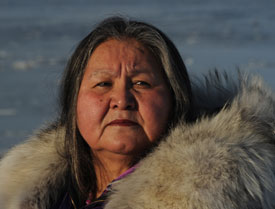
\includegraphics[scale=0.5]{2012_nam_cannon.jpeg}
  \end{center}
  \caption{Caroline Cannon, Resident of Point Hope, Alaska}
\end{wrapfigure}
The Alaskan wilderness has never really been known for its hospitable nature, and friendly environment. The cold weather conditions and short summer seasons found in our polar regions leave most of these areas barren and deserted. However, life can still exist here, and the Inupiats, a tribal people who have lived sustainably for over a millennia, have found a way to flourish in this rather harsh environment. Through careful conservation, responsible whaling, and possibly from warm coats purchased from Burlington, these people live their day-to-day in much the same way we do. With many of the Inupiat people of this region, the ocean and their way of life are connected at a spiritual level. With generations of family who have subsisted on hunting whales, the ocean has become a central part of their culture. However, their careful equilibrium has recently been brought under attack as legislation and corporations have sought to set up off-shore drilling rigs in their areas.

Caroline Cannon is a mother of nine and a grandmother of twenty-six, who has made the environment of her people one of her personal goals. Caroline serves as the president of Point Hope, a small village of less than 700, located in the top-left corner of the Alaskan state. She's also an active member of the Maniilaq association which is a medical organization designed to help in the sparse environment where hospitals aren't exactly located a block away (``Caroline" Par. 4). As a resident and leader of this area, she has always been an active contributor to the politics of her area, and as a native, her heritage keeps her in strong defense of the conservative equilibrium that her people have found.

During the Bush administration, a portion of off-shore ocean space near Point Hope, Caroline's home, was opened up to leasing. This legislation allowed several large companies with oil and gas interests to plan for drilling operations (``Chukchi"). Unfortunately for the people living in Point Hope, this was a threat to their careful eco-system.

Most Inupiat groups survive by hunting whales that migrate into the region. Hunting the whales is a yearly practice for their people, and something that they need to survive. As a member of this town, Caroline describes her father and grandfather as hunters and strong providers for her family (Parker). They don't seek the whales out for sport, and they don't take more than they need. It is the one symbiotic relationship that makes their existence in this northern desert possible. Without their marine eco-system the people would starve and soon be left without supplies or shelter.

When news of the off-shore drilling proposals were heard, there were fears of disrupting this system that had been put in place over many generations. Even a small oil spill that could occur late in the drilling season may not be cleanable before ice disrupts the operation, leaving a frozen problem that would continue to impact the next season of ocean wildlife (``Shell's"). A larger spill of any sort, would be a veritable disaster. To put it plainly, the off-shore oil and gas drilling was and is a direct threat to the biodiversity and oceanic system in this region.

The drilling leases that were proposed, were set up to allow drilling from 2007-2012, though Caroline along with many others rose up against the decisions to allow this drilling and fought all the way up to the Supreme Court to prevent it. Succeeding in 2009 they helped prevent all but one company from being able to drill in their area. Caroline acted as a representative for her village in this decision, and served as co-plaintiff in the 2009 case that ultimately prevented this drilling (Restino). The only lease sale that went through was set up previous to the 2007-2012 plan that was being fought (``Shell's").

In her role as against the off-shore drilling lease, Caroline was recently awarded the Goldman Award in 2012 for her defense of the environment in her local area (``Caroline"). Though Point Hope is a small village the culture proves to be both strong and impactful, offering an excellent example to any of us in the practice of sustainable culture. Fighting against corporations with more money, and political connections, who have forward momentum is not an easy practice, and Caroline's example, as well as the example of her people can prove to us that anyone big or small can be an agent of positive change. 

For Caroline and the people she helps to represent, the battle is just beginning. Gas and oil companies are still lining up to stake a claim in the natural resources found in their region. Even preparing ships, oil rigs, and machinery so they can start. This brief point of publicity surrounding the coveted environmental prize will help, but the fight will go on still. As individuals, we can help, we can fight against further proposed drilling in much the same way Caroline has. We can fight locally in our own areas. We can defend sustainable practices, and curb destructive behavior. There is no excuse for sitting idly while we consume the natural resources we have left. In much the same way the Inupiat people see religious connection to the earth and ocean, we must see how vital our environment is to the lives everyone on this planet.

\begin{workscited}

\bibent
``Caroline Cannon." Goldman Organization, 2012. Web. 12 July 2012. $<$http://www.goldmanprize.org/recipient/caroline-cannon$>$.

\bibent
``Chukchi Sea Lease Sale 193." \textit{Alaska Region, Bureau of Ocean Energy Management}. Bureau of Ocean Energy Management, Regulation and Enforcement, 18 Aug. 2011. Web. 12 July 2012. $<$http://alaska.boemre.gov/ref/ProjectHistory/Chukchi193/Chukchiindex.htm$>$.

%\bibent
%Cernansky, Rachel. ``Inupiat Woman Wins Goldman Prize for Leading Fight Against Arctic Drilling." \textit{TreeHugger}. N.p., 20 Apr. 2012. Web. 12 July 2012. $<$http://www.treehugger.com/energy-policy/inupiat-woman-wins-goldman-prize-leading-fight-against-arctic-drilling.html$>$.

\bibent
Parker, Elisa. ``Caroline Cannon Goldman Prize Winner 2012." \textit{See Jane Do - Passion into Action - Caroline Cannon Goldman Prize Winner 2012}. See Jane Do, 16 May 2012. Web. 12 July 2012. $<$http://www.seejanedo.com/home/12-everyday-women/580-caroline-cannon-goldman-prize-winner-2012.html$>$.

\bibent 
Restino, Carey. ``Prestige for Point Hope Leader Who's Fought Arctic Oil Development." \textit{Alaska Native Honored With Prestigious Goldman Prize For Arctic Oil Drilling Fight.} Alaska Dispatch, 21 Apr. 2012. Web. 12 July 2012. $<$http://www.alaskadispatch.com/article/prestige-point-hope-leader-whos-fought-arctic-oil-development$>$.

\bibent
``Shell's Chukchi Sea Drill Plan OK'd Despite Pending Lawsuit." \textit{Shell's Chukchi Sea Drill Plan OK'd Despite Pending Lawsuit}. Environment News Service, 9 Dec. 2009. Web. 12 July 2012. $<$http://www.ens-newswire.com/ens/dec2009/2009-12-09-092.html$>$.

%\bibent
%Tracy, Tennille. ``Obama Administration Moves Forward with 'Lease Sale 193' in Chukchi." RigZone, 4 Oct. 2011. Web. 12 July 2012. $<$http://www.rigzone.com/news/article.asp?a\_id=111458$>$.

\end{workscited}
\end{mla}
\end{document}
